\documentclass[tikz,border=5]{standalone}
\usetikzlibrary{graphs,arrows.meta,arrows, positioning, automata}

\begin{document}

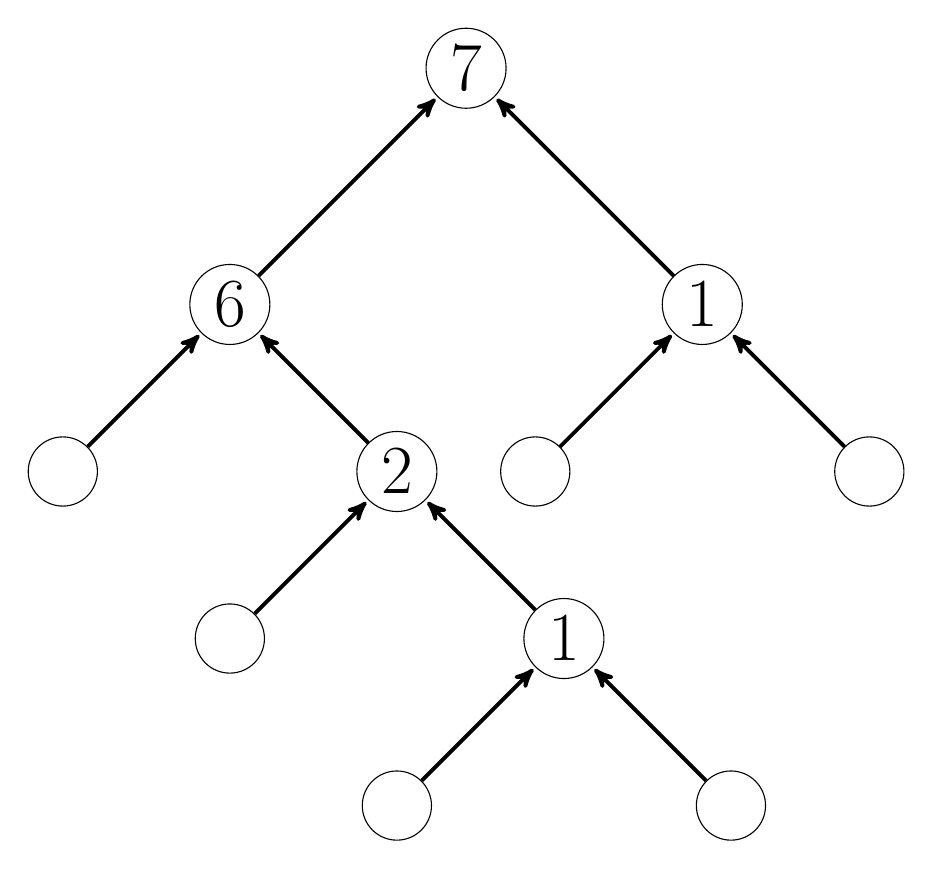
\begin{tikzpicture}[>=stealth',shorten >=1pt,node distance=3cm,on grid,initial/.style={}]
    \node[state] (T7) at (0,0) {\Huge $7$};
    \node[state] (T6) at (-3,-3) {\Huge $6$};
    \node[state] (T1_1) at (3,-3) {\Huge $1$};
    \node[state] (T6_C1) [below left =of T6] {};
    \node[state] (T2) [below right=of T6] {\Huge $2$};
    \node[state] (T1_1_C1) [below left =of T1_1] {};
    \node[state] (T1_1_C2) [below right=of T1_1] {};
    \node[state] (T2_C1) [below left =of T2] {};
    \node[state] (T1_2) [below right=of T2] {\Huge $1$};
    \node[state] (T1_2_C1) [below left =of T1_2] {};
    \node[state] (T1_2_C2) [below right=of T1_2] {};

    \tikzset{mystyle/.style={->,double=black}}
    %\tikzset{every node/.style={fill=white}}
    \path (T6) edge [mystyle] node {} (T7);
    \path (T1_1) edge [mystyle] node {} (T7);
    \path (T6_C1) edge [mystyle] node {}  (T6);
    \path (T2) edge [mystyle] node {}  (T6);
    \path (T1_1_C1) edge [mystyle] node {}  (T1_1);
    \path (T1_1_C2) edge [mystyle] node {}  (T1_1);
    \path (T2_C1) edge [mystyle] node {}  (T2);
    \path (T1_2) edge [mystyle] node {}  (T2);
    \path (T1_2_C1) edge [mystyle] node {}  (T1_2);
    \path (T1_2_C2) edge [mystyle] node {}  (T1_2);

\end{tikzpicture}

\end{document}